\section{Compressed Sensing with Coordinate Descent}
The most basic cd algorithm for image reconstruction

Tries to minimize the L1 norm of the image

\begin{equation}
	\underset{X}{minimize} \: \left \| V - F^{-1}X \right \|_2^2 + \lambda \left \| X \right \|_1 \\
\end{equation}

\begin{lstlisting} 
def coordinate_descent(V_residual, X, lambda):
	for i in pixels_row:
		for j in pixels_column:
			x_old = X[i, j]
			fourier_column = calculate_fourier_transform(i, j)
			fr = real(fourier_column)
			fi = imag(fourier_column)
			rr = real(V_residual)
			ri = imag(V_residual)
			
			#find apex
			a = sum(fr**2 + 2*fr*fi + fi**2)
			b = sum(fr*rr + fr*ri + fi*rr + fi*ri)
			x_new = b / a + x_old
			
			x_new = shrink(x_new, lambda)
			X[i, j] = x_new
			V_residual = V_residual - fourier_column * (x_new - x_old)
\end{lstlisting}\label{cd:basic}

How the algorithm works, shrinkage. 

Good points: Uses exact fourier transform. Assuming all other coordinates are fixed, we find the optimum. If the coordinates are independent, we converge faster. Heuristics can be used.

If we do not reconstruct the image $X$ directly, but in a different space. In this work, starlets were used. The next section \ref{cd:starlets} describes starlets in more detail.

Calculates the full Fourier Transformation matrix. Only changes a subset of the image. Active set heuristic after a full run. This is still impractical for meerKAT data size. Since we use starlets, there is a heuristic where we never need to calculate the full Matrix $F^{-1}$. This heuristic is described in section \ref{cd:heuristic}



\subsection{Starlets Regularization} \label{cd:starlets}
Starlet is a multi-scale wavelet representation which were specifically developed for astronomy.

Over-complete representation. More starlets than there are pixels. Sparse representation, the number of non-zero starlets is smaller than the number of pixels

Starlets as a series of convolutions.

Forward transform, from image to starlets

From Starlets to image

\subsection{Active set heuristic with Starlets}\label{cd:heuristic}
Even though the starlets are an over-complete dictionary, they have an approximate transform from image to starlet space. For Coordinate Descent, this can be used as a active set heuristic: We try to find the coefficients which are likely to be non-zero. This helps us so we do not need to calculate the whole matrix product $F^{-1}D$. We only use columns that are likely to be not zero.

\begin{figure}[h]
	\centering
	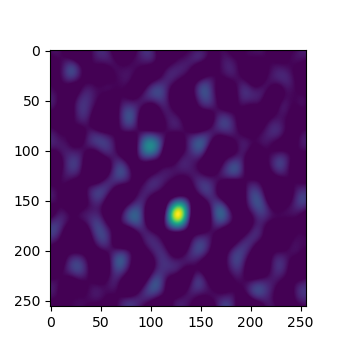
\includegraphics[width=0.5\linewidth]{./chapters/05.algorithms/sim02/starlets0.png}
	\caption{Starlet Level 0}
	\label{alg:heuristic:starlet}
\end{figure}

The higher the number, the more likely this component is to be non-zero. It is essentially a probability distribution for which starlet components are non-zero.

Stupid approach with line search. Could be done more efficiently by using the histogram of the starlet level.

\subsection{Implementation}
coordinate descent with active set heuristic

